%% SECTION HEADER /////////////////////////////////////////////////////////////////////////////////////
\section{Structures mesh generation for the \acs{fcgm}}
\label{sec:honeycomb}

%% SECTION CONTENT ////////////////////////////////////////////////////////////////////////////////////
The modelled structure is composed of the following components: 2D for the core, epoxy adhesive and cyanoacrylate glue and 3D for the \ac{cfrp} plate and \acp{pzt}.
During the creation of the core mesh, special attention was taken to minimised the number of non-zero values in the matrix \(\textbf{G}\).
The core elements were selected for the slave mesh, with one spectral element dedicated to each honeycomb cell wall.
The master meshes of the skin panel and adhesive layer were divided by three rhombic elements into the area under the core cell.
This way, the interface nodes coincide with those on the hexagon edges (red line in Fig.~\ref{fig:skin_mesh}(\textbf{b})).

The mesh for the cyanoacrylate adhesive consisted of five elements, with a second-order curve at the structure boundary as it is presented in Fig.~\ref{fig:skin_mesh}(\textbf{c}).
This structure was connected to the skin with the non-matching interface elements with the adhesive mesh chosen as a slave one.
The \ac{pzt} mesh coincides with the glue mesh and they are connected with the matching interface elements.
\begin{figure}[H]
	\begin{center}
		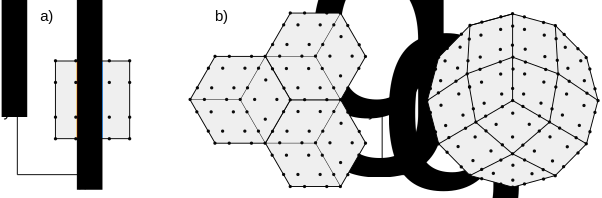
\includegraphics[width=0.95\textwidth]{Chapter_5/skin_mesh}
	\end{center}
	\caption{The mesh with the node distribution, (\textbf{a}) spectral element used for modeling the wall of the core, (\textbf{b}) excerpt of the skin plate and (\textbf{c}) cyanoacrylate glue mesh with the second-order curve at the boundary.}
	\label{fig:skin_mesh}
\end{figure}

The number of nodes for the particular elements are as follows: the core \(6 \times 5\), epoxy adhesive and cyanoacrylate glue \numproduct{6 x 6}, the plate \numproduct{6 x 6 x 4} and \acp{pzt} \numproduct{6 x 6 x 3}.
While the maximum length of the skin element is 6 \unit{\mm}, such a \ac{cfrp} model satisfies the condition of at least six nodes per wavelength for the \ac{a0}, as it is the shortest mode propagating in the assumed frequency range.
Table~\ref{tab:wavelength} shows the \ac{a0} wavelengths for various frequency and propagation angles.
\begin{table}[H]
	\small
	\tabcolsep=0.75cm
	%\centering
	\caption{\label{tab:wavelength}The wavelength of the \ac{a0} mode propagated in the presented \ac{cfrp} plate.}
	\begin{tabular}{cccccc}
		\toprule
		\textbf{Frequency} & \multicolumn{5}{c}{\textbf{Propagation angle}}\\
		\unit{\kHz} & \ang{0} & \ang{30} & \ang{45} & \ang{60} & \ang{90}\\
		\midrule
		50 & 16.5& 15.2&15.0&15.2&16.6\\
		100 & 10.3& 9.6&9.5&9.6&10.3\\
		150 & 7.5& 7.1&7.0&7.1&7.5\\
		\bottomrule
		\multicolumn{6}{r}{{\scriptsize{source: Dispersion Calculator v1.9}}}
	\end{tabular}
\end{table}